\documentclass[journal]{new-aiaa}
\usepackage[utf8]{inputenc}

\usepackage{graphicx}
\usepackage{subcaption}
\usepackage{amsmath}
\usepackage[version=4]{mhchem}
\usepackage{siunitx}
\usepackage{float}
\usepackage{array}
\usepackage[export]{adjustbox}
\usepackage{longtable, tabularx}
\usepackage{tabulary}
\usepackage{graphicx,color}
\usepackage{atbegshi,picture}
\usepackage{color, colortbl}
\graphicspath{ {./Figures/} }
\setlength\LTleft{0pt} 

\title{Gazebo Factory Pick and Place Simulation}
        
\author{Jacob T. Cassady, Rohan Chandra}
\affil{Johns Hopkins University, Whiting School of Engineering, Baltimore, MD, 21206}

\begin{document}

\maketitle
\begin{abstract}
    The goal of this paper is to present the design and analysis of a pick and place simulation using ROS 2 Jazzy \cite{doi:10.1126/scirobotics.abm6074} and Gazebo Harmonic \cite{Gazebo}.
\end{abstract}

\section{Introduction}\label{sec:Introduction}
This paper explores the development of a factory robot. 
The robot, a UR20 from Universal Robotics, was tasked with picking up an object off of a table and then placing it onto a four wheeled robot, specifically the Husky A300 from Open Robotics. 
ROS2, and more specifically the Moveit library \cite{DBLP:journals/corr/ColemanSCC14}, was used to implement the equations of motions for the arm. 
The process by which these equations of motion were derived are explored later in this report. 
Gazebo was the tool of choice for simulating the environment, which included the UR20, the Husky A300, and the factory within which these robots lived. 
More information about the chosen hardware is described in Section \ref{sec:Robot Design}, while information about the simulation configuration is detailed in Section \ref{sec:Simulation Design}.
Section \ref{sec:Control Software} overviews the software implemented to control the robot in simulation.

This project was appealing given how applicable it is to the real world. 
Robots like the UR20 and the Husky are increasingly becoming integral parts of day-to-day factory workflows. 
One can imagine a UR20 picking up any number of items and placing them on a four-wheeled robot, and then that robot moving autonomously to transport its goods to either the next stage of production or to be shipped.

\section{Robot Design}\label{sec:Robot Design}

Section \ref{sec:Robot Design:Hardware} describes the hardware chosen for the pick and place task.
Section \ref{sec:Robot Design:Equations of Motion} details the equations of motion for the UR20.

\subsection{Hardware}\label{sec:Robot Design:Hardware}

The UR20 is a robotic arm from Universal Robotics, designed to be incorporated into a traditional factory. 
It is capable of lifting up to 25 kg of weight, and is capable of performing a variety of tasks including palletizing, welding, and (most relevant for this project), material handling. 
It was this last quality in particular that led to it being used for this project. 
To enable this robot to pick up a block, it was given a Robotiq 85 Gripper, manufactured by Robotiq Inc. 
This robotic hand is extremely versatile, due in part to its use of a Distal Phalanx and Proximal Phalanx. 
These two components are flexible, and as such, can grip onto differently shaped objects, such as cylinders and cubes, with equal dexterity and strength. 
Given the hand's versatility, it felt the most realistic to use for this project. 

\begin{figure}[H]
    \centering
    \begin{subfigure}{0.45\textwidth}
        \centering
        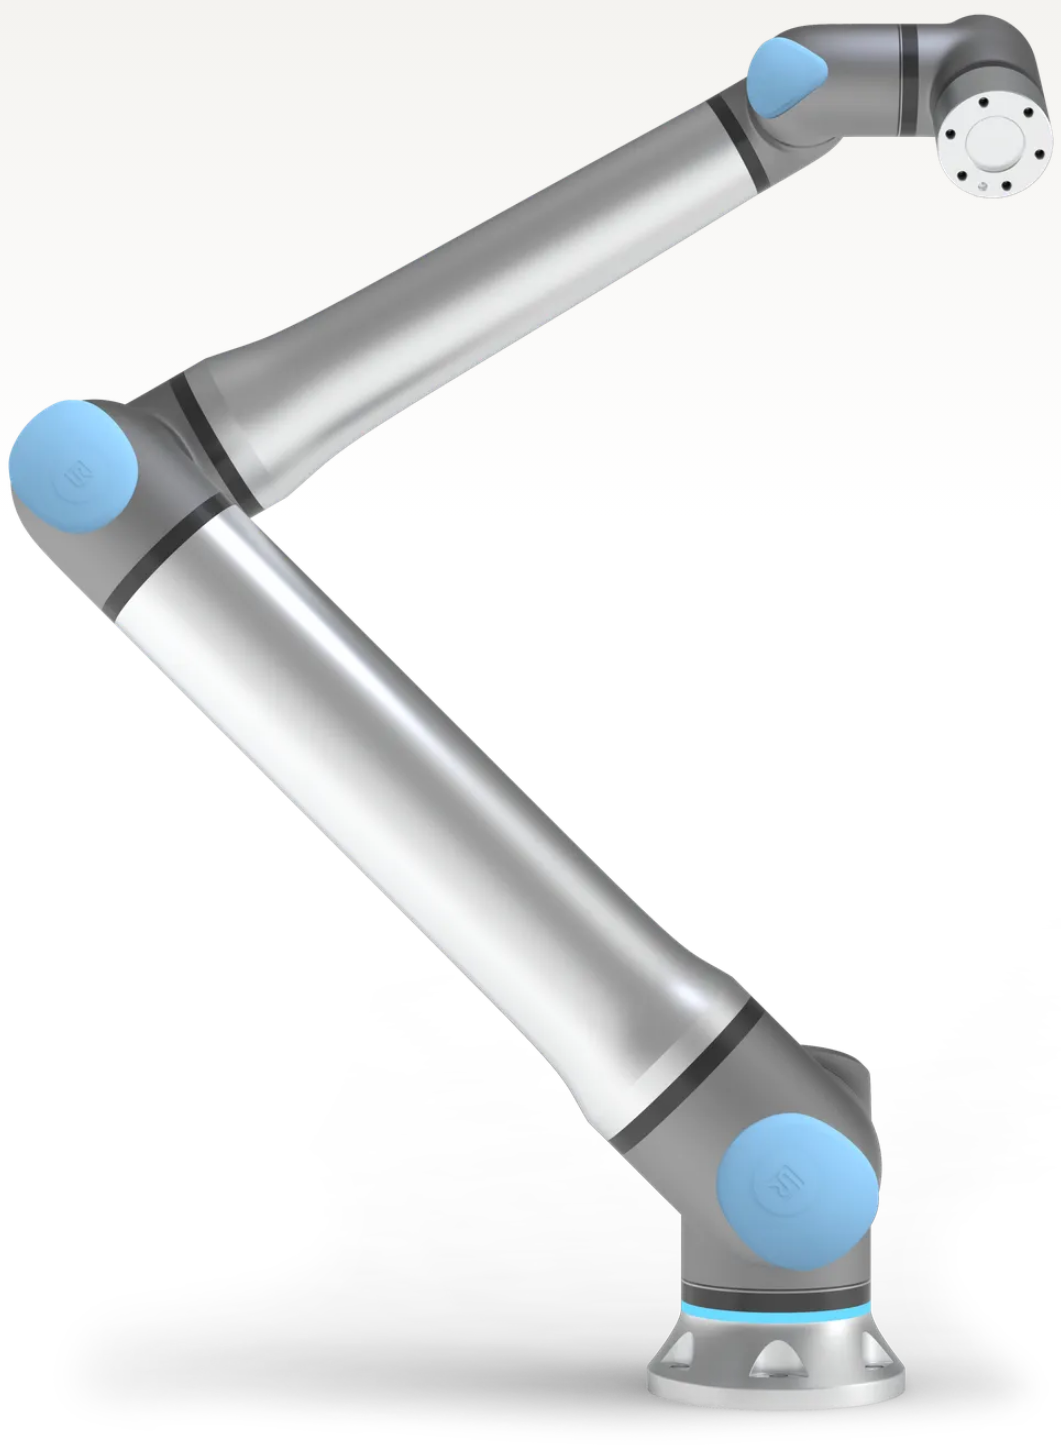
\includegraphics[width=\textwidth]{UR.PNG}
        \caption{UR20 \cite{UR20}}
        \label{fig:UR20}
    \end{subfigure}
    \hfill
    \begin{subfigure}{0.45\textwidth}
        \centering
        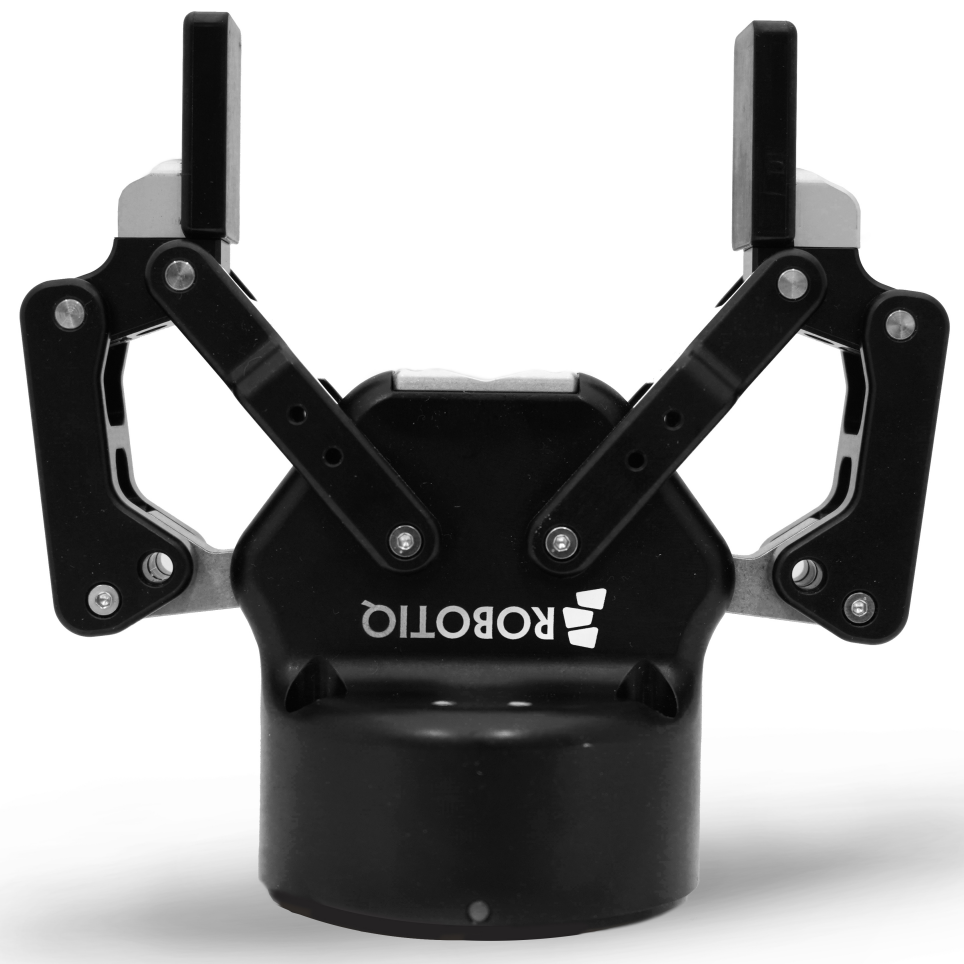
\includegraphics[width=\textwidth]{Robotiq_85.PNG}
        \caption{Robotiq 85 Gripper \cite{robotiq2020grippers}}
        \label{fig:Robotiq 85 Gripper}
    \end{subfigure}
    \caption{Side-by-side view of UR20 and Robotiq 85 Gripper.}
    \label{fig:side_by_side}
\end{figure}

\subsection{Equations of Motion}\label{sec:Robot Design:Equations of Motion}
A python script was created to calculate the equations of motion for the UR20 robot.
The full script is included in the appendix while some important sections have been included when pertinent.

\subsubsection{Denavit-Hartenberg Parameters}\label{sec:Equations of Motion:DH}

Denavit-Hartenberg parameters for the UR20 robot were obtained from Universal Robots documentation \cite{UR20DH}.
A diagram of the frame for each link is shown in figure \ref{fig:UR DH Diagram} and a table of the Denavit-Hartenberg parameters is shown in Table \ref{tab:DH Table}.
The diagram is the same for every UR robot, but the values of $d_i$ and $a_i$ are dependent on the model.
Note: although figure \ref{fig:UR DH Diagram} labels their links as Link 0 to Link 5, this paper will refer to them as Link 1 to Link 6.

\begin{figure}[H]
    \centering
    \begin{minipage}{0.45\textwidth}
        \centering
        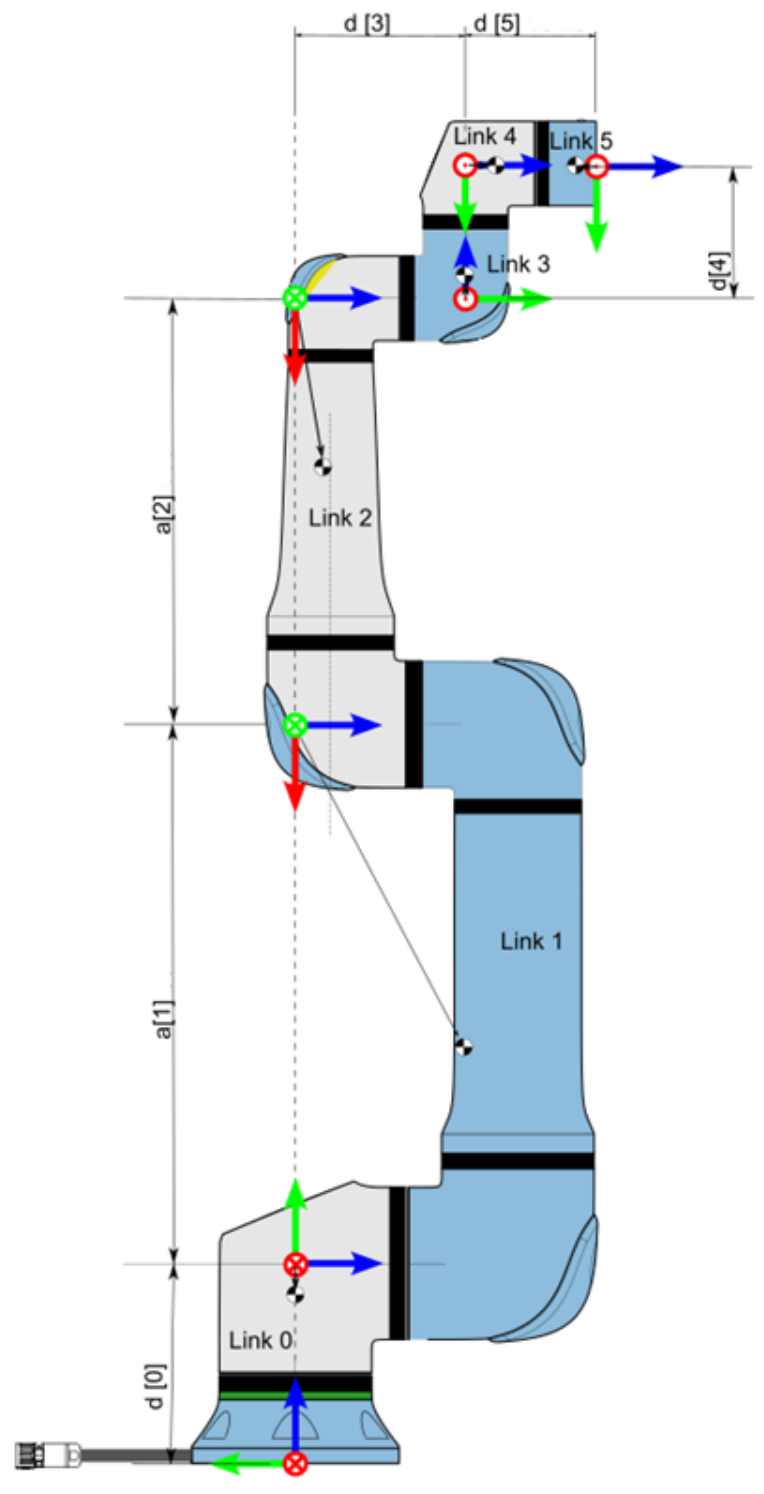
\includegraphics[width=\textwidth]{UR_Diagram.PNG}
        \caption{UR20 DH Diagram \cite{UR20DH}}
        \label{fig:UR DH Diagram}
    \end{minipage}
    \hfill
    \begin{minipage}{0.45\textwidth}
        \centering
        \begin{tabular}{|c|c|c|c|c|}
          \hline
          Link & \(\theta_i\) & \(d_i\) & \(a_i\) & \(\alpha_i\) \\
          \hline
          1 & $\theta_1^*$ & $0.2363$ & 0         & $\frac{\pi}{2}$ \\
          2 & $\theta_2^*$ &      $0$ & $-0.8620$ & 0 \\
          3 & $\theta_3^*$ &      $0$ & $-0.7287$ & 0 \\
          4 & $\theta_4^*$ & $0.2010$ & 0         & $\frac{\pi}{2}$ \\
          5 & $\theta_5^*$ & $0.1593$ & 0         & $-\frac{\pi}{2}$ \\
          6 & $\theta_6^*$ & $0.1543$ & 0         & 0 \\
          \hline
        \end{tabular}
        \captionof{table}{DH Table \cite{UR20DH}}
        \label{tab:DH Table}
    \end{minipage}
\end{figure}

\subsubsection{Homogenous Transforms}\label{sec:Equations of Motion:DH:Homogenous Transforms}

Homogenous Transformation matrices were calculated using the Denavit-Hartenberg parameters and equation \ref{eq:A_i} from Spong \cite{spong2020robot}.

\begin{equation}\label{eq:A_i}
    A_i = \begin{bmatrix}
        c_{\theta_i} & -s_{\theta_i}c_{\alpha_i} & s_{\theta_i}s_{\alpha_i} & a_ic_{\theta_i} \\
        s_{\theta_i} & c_{\theta_i}c_{\alpha_i}  & -c_{\theta_i}s_{\alpha_i} & a_is_{\theta_i} \\
        0              & s_{\alpha_i}                & c_{\alpha_i}                & d_i \\
        0              & 0                             & 0                             & 1
    \end{bmatrix}
\end{equation}

\begin{center}
    \begin{tabular}{ccc}
    \(
    A_1 =
    \begin{bmatrix}
        c_{\theta_1^*} & 0 & s_{\theta_1^*} & 0 \\
        s_{\theta_1^*} & 0 & -c_{\theta_1^*} & 0 \\
        0 & 1 & 0 & 0.2363 \\
        0 & 0 & 0 & 1
    \end{bmatrix}
    \)
    &
    \(
    A_2 =
    \begin{bmatrix}
        c_{\theta_2^*} & -s_{\theta_2^*} & 0 & -0.862 c_{\theta_2^*} \\
        s_{\theta_2^*} & c_{\theta_2^*} & 0 & -0.862 s_{\theta_2^*} \\
        0 & 0 & 1 & 0 \\
        0 & 0 & 0 & 1
    \end{bmatrix}
    \)
    &
    \(
    A_3 =
    \begin{bmatrix}
    c_{\theta_3^*} & -s_{\theta_3^*} & 0 & -0.7287 s_{\theta_3^*} \\
    s_{\theta_3^*} & c_{\theta_3^*} & 0 & -0.7287 s_{\theta_3^*} \\
    0 & 0 & 1 & 0 \\
    0 & 0 & 0 & 1
    \end{bmatrix}
    \) 
    \\
    \(
    A_4 =
    \begin{bmatrix} 
        c_{\theta_4^*} & 0 & s_{\theta_4^*} & 0 \\ 
        s_{\theta_4^*} & 0 & -c_{\theta_4^*} & 0 \\ 
        0 & 1 & 0 & 0.201 \\ 
        0 & 0 & 0 & 1 
    \end{bmatrix}
    \)
    &
    \(
    A_5 =
    \begin{bmatrix} 
        c_{\theta_5^*} & 0 & -s_{\theta_5^*} & 0 \\ 
        s_{\theta_5^*} & 0 & c_{\theta_5^*} & 0 \\ 
        0 & -1 & 0 & 0.1593 \\ 
        0 & 0 & 0 & 1 \end{bmatrix}
    \)
    &
    \(
    A_6 =
    \begin{bmatrix} 
        c_{\theta_6^*} & -s_{\theta_6^*} & 0 & 0 \\ 
        s_{\theta_6^*} & c_{\theta_6^*} & 0 & 0 \\ 
        0 & 0 & 1 & 0.1543 \\ 
        0 & 0 & 0 & 1 
    \end{bmatrix}
    \)
    \end{tabular}
\end{center}

\begin{description}
    \item[$T_0^1=A_1$] \hfill
    $$
    T_0^1 =
    \begin{bmatrix}
        c_{\theta_1^*} & 0 & s_{\theta_1^*} & 0 \\
        s_{\theta_1^*} & 0 & -c_{\theta_1^*} & 0 \\
        0 & 1 & 0 & 0.2363 \\
        0 & 0 & 0 & 1
    \end{bmatrix}
    $$

    \item[$T_0^2=A_1A_2$] \hfill

    $$
    T_0^2 = \begin{bmatrix}
        c_{\theta_1^*}c_{\theta_2^*} & -s_{\theta_2^*}c_{\theta_1^*} & s_{\theta_1^*} & -0.862c_{\theta_1^*}c_{\theta_2^*} \\
        s_{\theta_1^*}c_{\theta_2^*} & -s_{\theta_1^*}s_{\theta_2^*} & -c_{\theta_1^*} & -0.862s_{\theta_1^*}c_{\theta_2^*} \\
        s_{\theta_2^*} & c_{\theta_2^*} & 0 & 0.2363-0.862 s_{\theta_2^*} \\
        0 & 0 & 0 & 1        
    \end{bmatrix}
    $$

    \item[$T_0^3=A_1A_2A_3$] \hfill

    $$
    T_0^3 = \begin{bmatrix}
        c_{\theta_1^*}c_{\theta_2^*+\theta_3^*} & -s_{\theta_2^*+\theta_3^*}c_{\theta_1^*} & s_{\theta_1^*} & -c_{\theta_1^*}(0.862c_{\theta_2^*}+0.7287c_{\theta_2^*+\theta_3^*}) \\
        s_{\theta_1^*}c_{\theta_2^*+\theta_3^*} & -s_{\theta_1^*}s_{\theta_2^*+\theta_3^*} & -c_{\theta_1^*} & -s_{\theta_1^*}(0.862c_{\theta_2^*}+0.7287c_{\theta_2^*+\theta_3^*}) \\
        s_{\theta_2^*+\theta_3^*} & c_{\theta_2^*+\theta_3^*} & 0 & 0.2363-0.862 s_{\theta_2^*} -0.7287 s_{\theta_2^*+\theta_3^*} \\
        0 & 0 & 0 & 1        
    \end{bmatrix}
    $$

    \item[$T_0^4=A_1A_2A_3A_4$] \hfill

    $$
    T_0^4 = \begin{bmatrix}
        c_{\theta_1^*}c_{\theta_2^*+\theta_3^*+\theta_4^*} & s_{\theta_1^*} & s_{\theta_2^*+\theta_3^*+\theta_4^*}c_{\theta_1^*} & -c_{\theta_1^*}(0.862c_{\theta_2^*}+0.7287c_{\theta_2^*+\theta_3^*})-0.201s_{\theta_1} \\
        s_{\theta_1^*}c_{\theta_2^*+\theta_3^*+\theta_4^*} & -c_{\theta_1^*} & s_{\theta_1^*}s_{\theta_2^*+\theta_3^*+\theta_4^*} & -s_{\theta_1^*}(0.862c_{\theta_2^*}+0.7287c_{\theta_2^*+\theta_3^*})-0.201c_{\theta_1} \\
        s_{\theta_2^*+\theta_3^*+\theta_4^*} & 0 & -c_{\theta_2^*+\theta_3^*+\theta_4^*} & 0.2363-0.862 s_{\theta_2^*} -0.7287 s_{\theta_2^*+\theta_3^*} \\
        0 & 0 & 0 & 1        
    \end{bmatrix}
    $$

    \item[$T_0^5=A_1A_2A_3A_4A_5$] \hfill

    $$
    T_0^5 = \begin{bmatrix}
        r_{11}^5 & r_{12}^5 & r_{13}^5 & r_{14}^5 \\
        r_{21}^5 & r_{22}^5 & r_{23}^5 & r_{24}^5 \\
        r_{31}^5 & r_{32}^5 & r_{33}^5 & r_{34}^5 \\
        0 & 0 & 0 & 1
    \end{bmatrix}
    $$

    \begin{align*}
        r_{11}^5 &= s_{\theta_1^*}s_{\theta_5^*} + c_{\theta_1^*}c_{\theta_2^*+\theta_3^*+\theta_4^*} \\
        r_{12}^5 &= -c_{\theta_1^*}s_{\theta_2^*+\theta_3^*+\theta_4^*} \\
        r_{13}^5 &= s_{\theta_1^*}c_{\theta_5^*}-c_{\theta_1^*}s_{\theta_5^*}c_{\theta_2^*+\theta_3^*+\theta_4^*} \\
        r_{14}^5 &= -c_{\theta_1^*}(0.862c_{\theta_2^*}+0.7287c_{\theta_2^*+\theta_3^*})-0.201s_{\theta_1} + 0.1593 c_{\theta_2^*+\theta_3^*\theta_4^*} c_{\theta_1^*} \\
        r_{21}^5 &= s_{\theta_1^*}c_{\theta_2^*+\theta_3^*+\theta_4^*}-s_{\theta_1^*}s_{\theta_5^*} \\
        r_{22}^5 &= -s_{\theta_1^*}s_{\theta_2^*+\theta_3^*+\theta_4^*} \\
        r_{23}^5 &= -c_{\theta_1^*}c_{\theta_5^*}-s_{\theta_1^*}s_{\theta_5^*}c_{\theta_2^*+\theta_3^*+\theta_4^*}\\
        r_{24}^ 5&= -s_{\theta_1^*}(0.862c_{\theta_2^*}+0.7287c_{\theta_2^*+\theta_3^*})-0.201c_{\theta_1} + 0.1593 c_{\theta_2^*+\theta_3^*\theta_4^*} s_{\theta_1^*}\\
        r_{31}^5 &= s_{\theta_2^*+\theta_3^*+\theta_4^*}c_{\theta_5^*} \\
        r_{32}^5 &= c_{\theta_2^*+\theta_3^*+\theta_4^*} \\
        r_{33}^5 &= -s_{\theta_5^*}s_{\theta_2^*+\theta_3^*+\theta_4^*} \\
        r_{34}^{5}&= 0.2363-0.862 s_{\theta_2^*} -0.7287 s_{\theta_2^*+\theta_3^*} - 0.1593 c_{\theta_2^*+\theta_3^*\theta_4^*} \\
    \end{align*}

    \item[$T_0^6=A_1A_2A_3A_4A_5A_6$] \hfill

    $$
    T_0^6 = \begin{bmatrix}
        r_{11}^6 & r_{12}^6 & r_{13}^6 & r_{14}^6 \\
        r_{21}^6 & r_{22}^6 & r_{23}^6 & r_{24}^6 \\
        r_{31}^6 & r_{32}^6 & r_{33}^6 & r_{34}^6 \\
        0 & 0 & 0 & 1
    \end{bmatrix}
    $$

    \begin{align*}
        r_{11}^6 &= c_{\theta_6^*}(s_{\theta_1^*}s_{\theta_5^*} + c_{\theta_1^*}c_{\theta_5^*}c_{\theta_2^*+\theta_3^*+\theta_4^*}) - c_{\theta^*_1}s_{\theta_6^*}s_{\theta_2^*+\theta_3^*+\theta_4^*} \\
        r_{12}^6 &= c_{\theta^*_6}(c_{\theta^*_1} c_{\theta^*_5} c_{\theta^*_2+\theta^*_3+\theta^*_4} + s_{\theta^*_1} s_{\theta^*_5}) - c_{\theta^*_1} s_{\theta^*_6} s_{\theta^*_2+\theta^*_3+\theta^*_4} \\
        r_{13}^6 &= -s_{\theta^*_6}(c_{\theta^*_1} c_{\theta^*_5} c_{\theta^*_2+\theta^*_3+\theta^*_4} - s_{\theta^*_1} s_{\theta^*_5}) - c_{\theta^*_1} c_{\theta^*_6} s_{\theta^*_2+\theta^*_3+\theta^*_4} \\
        r_{14}^6 &= -c_{\theta_1^*}(0.862c_{\theta_2^*}+0.7287c_{\theta_2^*+\theta_3^*})-0.201c_{\theta_1} + 0.1593 s_{\theta_2^*+\theta_3^*\theta_4^*} c_{\theta_1^*}-0.1543c_{\theta^*_1}s_{\theta^*_5}c_{\theta_2^*+\theta_3^*\theta_4^*}+0.1543s_{\theta^*_1}c_{\theta^*_5} \\
        r_{21}^6 &= c_{\theta_6^*}(-c_{\theta_1^*}s_{\theta_5^*} + s_{\theta_1^*}c_{\theta_5^*}c_{\theta_2^*+\theta_3^*+\theta_4^*}) - s_{\theta^*_1}s_{\theta_6^*}s_{\theta_2^*+\theta_3^*+\theta_4^*} \\
        r_{22}^6 &=  c_{\theta^*_6}(s_{\theta^*_1} c_{\theta^*_5} c_{\theta^*_2+\theta^*_3+\theta^*_4} - c_{\theta^*_1} s_{\theta^*_5}) - s_{\theta^*_1} s_{\theta^*_6} s_{\theta^*_2+\theta^*_3+\theta^*_4} \\
        r_{23}^6 &= -s_{\theta^*_6}(c_{\theta^*_1} s_{\theta^*_5} c_{\theta^*_2+\theta^*_3+\theta^*_4} - c_{\theta^*_1} s_{\theta^*_5}) - s_{\theta^*_1} c_{\theta^*_6} s_{\theta^*_2+\theta^*_3+\theta^*_4} \\
        r_{24}^6 &= -s_{\theta_1^*}(0.862c_{\theta_2^*}+0.7287c_{\theta_2^*+\theta_3^*})-0.201c_{\theta_1} + 0.1593 s_{\theta_2^*+\theta_3^*\theta_4^*} s_{\theta_1^*}-0.1543s_{\theta^*_1}s_{\theta^*_5}c_{\theta_2^*+\theta_3^*\theta_4^*}-0.1543c_{\theta^*_1}c_{\theta^*_5} \\
        r_{31}^6 &= c_{\theta^*_6}s_{\theta^*_2+\theta^*_3+\theta^*_4}c_{\theta^*_5}+s_{\theta^*_6}c_{\theta^*_2+\theta^*_3+\theta^*_4} \\
        r_{32}^6 &= -s_{\theta^*_6}s_{\theta^*_2+\theta^*_3+\theta^*_4}c_{\theta^*_5}+c_{\theta^*_6}c_{\theta^*_2+\theta^*_3+\theta^*_4} \\
        r_{33}^6 &= -s_{\theta_5^*}s_{\theta_2^*+\theta_3^*+\theta_4^*} \\
        r_{34}^6 &= 0.2363-0.862 s_{\theta_2^*} -0.7287 s_{\theta_2^*+\theta_3^*} - 0.1543 s_{\theta^*_5}s_{\theta_2^*+\theta_3^*+\theta_4^*} - 0.1593 c_{\theta_2^*+\theta_3^*+\theta_4^*} \\
    \end{align*}

\end{description}

\subsubsection{Jacobians for $c_1 \dots c_6$}\label{sec:Equations of Motion:Jacobians}

Center of Mass values were obtained from the UR20 documentation \cite{UR20DH} and are shown in Table \ref{tab:Link Physical Properties}.
Note these values are relative to the link frames not the base frame.
To find the center of mass relative to the base frame, the homogenous transformation matrix for each link was multiplied by the center of mass vector $O_{c_i}=T_0^i COM$.

\begin{table}[H]
    \centering
    \begin{tabular}{|c|c|c|c|}
      \hline
      Link & Mass [kg] & Center of Mass & Inertia Matrix \\
      \hline
      1 & $16.343$ & $\begin{bmatrix} 0 \\ -0.0610 \\ 0.0062 \end{bmatrix}$ & $\begin{bmatrix} 0.0887 & -0.0001 & -0.0001 \\
                                     -0.0001 &  0.0763 &  0.0072 \\
                                     -0.0001 &  0.0072 &  0.0842 \end{bmatrix}$ \\
      2 & $29.632$ & $\begin{bmatrix} 0.5226 \\ 0 \\ 0.2098 \end{bmatrix}$ & $\begin{bmatrix} 0.1467 & 0.0002 & -0.0516 \\
                                      0.0002 & 4.6659 &  0.0000 \\
                                     -0.0516 & 0.0000 &  4.6348 \end{bmatrix}$ \\
      3 & $7.879$ & $\begin{bmatrix} 0.3234 \\ 0 \\ 0.0604 \end{bmatrix}$ & $\begin{bmatrix} 0.0261 & -0.0001 & -0.0290 \\
                                     -0.0001 &  0.75763 &  0 \\
                                     -0.0290 &  0 &  0.7533 \end{bmatrix}$ \\
      4 & $3.054$ & $\begin{bmatrix} 0 \\ -0.0026 \\ 0.0393 \end{bmatrix}$ & $\begin{bmatrix} 0.0056 & 0 & 0 \\
                                     0 &  0.0054 &  0.0004 \\
                                     0 &  0.0004 &  0.0040 \end{bmatrix}$ \\
      5 & $3.126$ & $\begin{bmatrix} 0 \\ 0.0024 \\ 0.0379 \end{bmatrix}$ & $\begin{bmatrix} 0.0059 & 0 & 0 \\
                                     0 &  0.0058 & -0.0004 \\
                                     0 &  -0.0004 &  0.0043 \end{bmatrix}$ \\
      6 & $0.846$ & $\begin{bmatrix} 0 \\ -0.0003 \\ -0.0318 \end{bmatrix}$ & $\begin{bmatrix} 0.0009 & 0 & 0 \\
                                     0 & 0.0009 & 0 \\
                                     0 & 0 & 0.0012 \end{bmatrix}$ \\
      \hline
    \end{tabular}
    \caption{Link Physical Properties \cite{UR20DH}}
    \label{tab:Link Physical Properties}
\end{table}

\begin{description}
    \item[$J_{c_1}$] \hfill
    $$
    \begin{bmatrix}
        \hat{z}_0 \times (\hat{O}_{c_1} - \hat{O}_0) & 0 & 0 & 0 & 0 & 0 \\
        \hat{z}_0                                    & 0 & 0 & 0 & 0 & 0
    \end{bmatrix}
    $$

    $$\begin{matrix}0 & 0 & 0 & 0 & 0 & 0\\0 & 0 & 0 & 0 & 0 & 0\\0 & 0 & 0 & 0 & 0 & 0\\0 & 0 & 0 & 0 & 0 & 0\\0 & 0 & 0 & 0 & 0 & 0\\1 & 0 & 0 & 0 & 0 & 0\end{matrix}$$

    \item[$J_{c_2}$] \hfill
    $$
    \begin{bmatrix}
        \hat{z}_0 \times (\hat{O}_{c_2} - \hat{O}_0) & \hat{z}_0 \times (\hat{O}_{c_2} - \hat{O}_1) & 0 & 0 & 0 & 0 \\
        \hat{z}_0                                    & \hat{z}_1                                    & 0 & 0 & 0 & 0
    \end{bmatrix}
    $$

    $$\begin{matrix}0.0062 \cos{\left(\theta_{1} \right)} & 0.061 \cos{\left(\theta_{1} \right)} & 0 & 0 & 0 & 0\\0.0062 \sin{\left(\theta_{1} \right)} & 0.061 \sin{\left(\theta_{1} \right)} & 0 & 0 & 0 & 0\\0 & 0 & 0 & 0 & 0 & 0\\0 & \sin{\left(\theta_{1} \right)} & 0 & 0 & 0 & 0\\0 & - \cos{\left(\theta_{1} \right)} & 0 & 0 & 0 & 0\\1 & 0 & 0 & 0 & 0 & 0\end{matrix}$$

    \item[$J_{c_3}$] \hfill
    $$
    \begin{bmatrix}
        \hat{z}_0 \times (\hat{O}_{c_3} - \hat{O}_0) & \hat{z}_1 \times (\hat{O}_{c_3} - \hat{O}_1) & \hat{z}_2 \times (\hat{O}_{c_3} - \hat{O}_2) & 0 & 0 & 0 \\
        \hat{z}_0                                    & \hat{z}_1                                    & \hat{z}_2 & 0 & 0 & 0
    \end{bmatrix}
    $$

    $$\begin{matrix}0.3394 \sin{\left(\theta_{1} \right)} \cos{\left(\theta_{2} \right)} + 0.2098 \cos{\left(\theta_{1} \right)} & 0.3394 \sin{\left(\theta_{2} \right)} \cos{\left(\theta_{1} \right)} & - 0.5226 \sin{\left(\theta_{2} \right)} \cos{\left(\theta_{1} \right)} & 0 & 0 & 0\\0.2098 \sin{\left(\theta_{1} \right)} - 0.3394 \cos{\left(\theta_{1} \right)} \cos{\left(\theta_{2} \right)} & 0.3394 \sin{\left(\theta_{1} \right)} \sin{\left(\theta_{2} \right)} & - 0.5226 \sin{\left(\theta_{1} \right)} \sin{\left(\theta_{2} \right)} & 0 & 0 & 0\\0 & - 0.3394 \cos{\left(\theta_{2} \right)} & 0.5226 \cos{\left(\theta_{2} \right)} & 0 & 0 & 0\\0 & \sin{\left(\theta_{1} \right)} & \sin{\left(\theta_{1} \right)} & 0 & 0 & 0\\0 & - \cos{\left(\theta_{1} \right)} & - \cos{\left(\theta_{1} \right)} & 0 & 0 & 0\\1 & 0 & 0 & 0 & 0 & 0\end{matrix}$$

    \item[$J_{c_4}$] \hfill
    $$
    \begin{bmatrix}
        \hat{z}_0 \times (\hat{O}_{c_4} - \hat{O}_0) & \hat{z}_1 \times (\hat{O}_{c_4} - \hat{O}_1) & \hat{z}_2 \times (\hat{O}_{c_4} - \hat{O}_2) & \hat{z}_3 \times (\hat{O}_{c_4} - \hat{O}_3) & 0 & 0 \\
        \hat{z}_0                                    & \hat{z}_1                                    & \hat{z}_2                                    & \hat{z}_3 & 0 & 0
    \end{bmatrix}
    $$

    \[
        \resizebox{\textwidth}{!}{$
        \begin{matrix}0.862 \sin{\left(\theta_{1} \right)} \cos{\left(\theta_{2} \right)} + 0.4053 \sin{\left(\theta_{1} \right)} \cos{\left(\theta_{2} + \theta_{3} \right)} + 0.0604 \cos{\left(\theta_{1} \right)} & \left(0.862 \sin{\left(\theta_{2} \right)} + 0.4053 \sin{\left(\theta_{2} + \theta_{3} \right)}\right) \cos{\left(\theta_{1} \right)} & 0.4053 \sin{\left(\theta_{2} + \theta_{3} \right)} \cos{\left(\theta_{1} \right)} & - 0.3234 \sin{\left(\theta_{2} + \theta_{3} \right)} \cos{\left(\theta_{1} \right)} & 0 & 0\\0.0604 \sin{\left(\theta_{1} \right)} - 0.862 \cos{\left(\theta_{1} \right)} \cos{\left(\theta_{2} \right)} - 0.4053 \cos{\left(\theta_{1} \right)} \cos{\left(\theta_{2} + \theta_{3} \right)} & \left(0.862 \sin{\left(\theta_{2} \right)} + 0.4053 \sin{\left(\theta_{2} + \theta_{3} \right)}\right) \sin{\left(\theta_{1} \right)} & 0.4053 \sin{\left(\theta_{1} \right)} \sin{\left(\theta_{2} + \theta_{3} \right)} & - 0.3234 \sin{\left(\theta_{1} \right)} \sin{\left(\theta_{2} + \theta_{3} \right)} & 0 & 0\\0 & - 0.862 \cos{\left(\theta_{2} \right)} - 0.4053 \cos{\left(\theta_{2} + \theta_{3} \right)} & - 0.4053 \cos{\left(\theta_{2} + \theta_{3} \right)} & 0.3234 \cos{\left(\theta_{2} + \theta_{3} \right)} & 0 & 0\\0 & \sin{\left(\theta_{1} \right)} & \sin{\left(\theta_{1} \right)} & \sin{\left(\theta_{1} \right)} & 0 & 0\\0 & - \cos{\left(\theta_{1} \right)} & - \cos{\left(\theta_{1} \right)} & - \cos{\left(\theta_{1} \right)} & 0 & 0\\1 & 0 & 0 & 0 & 0 & 0\end{matrix}
        $}
    \]

    \item[$J_{c_5}$] \hfill
    $$
    \begin{bmatrix}
        \hat{z}_0 \times (\hat{O}_{c_5} - \hat{O}_0) & \hat{z}_1 \times (\hat{O}_{c_5} - \hat{O}_1) & \hat{z}_2 \times (\hat{O}_{c_5} - \hat{O}_2) & \hat{z}_3 \times (\hat{O}_{c_5} - \hat{O}_3) & \hat{z}_4 \times (\hat{O}_{c_5} - \hat{O}_4) & 0 \\
        \hat{z}_0                                    & \hat{z}_1                                    & \hat{z}_2                                    & \hat{z}_3                                    & \hat{z}_4 & 0
    \end{bmatrix}
    $$

    \[
        \resizebox{\textwidth}{!}{$
        \begin{matrix}\left(0.862 \cos{\left(\theta_{2} \right)} + 0.7287 \cos{\left(\theta_{2} + \theta_{3} \right)}\right) \sin{\left(\theta_{1} \right)} - 0.0393 \sin{\left(\theta_{1} \right)} \sin{\left(\theta_{2} + \theta_{3} + \theta_{4} \right)} + 0.1984 \cos{\left(\theta_{1} \right)} & \left(0.862 \sin{\left(\theta_{2} \right)} + 0.7287 \sin{\left(\theta_{2} + \theta_{3} \right)} + 0.0393 \cos{\left(\theta_{2} + \theta_{3} + \theta_{4} \right)}\right) \cos{\left(\theta_{1} \right)} & \left(0.7287 \sin{\left(\theta_{2} + \theta_{3} \right)} + 0.0393 \cos{\left(\theta_{2} + \theta_{3} + \theta_{4} \right)}\right) \cos{\left(\theta_{1} \right)} & 0.0393 \cos{\left(\theta_{1} \right)} \cos{\left(\theta_{2} + \theta_{3} + \theta_{4} \right)} & 0.00259 \cos{\left(\theta_{1} \right)} \cos{\left(\theta_{2} + \theta_{3} + \theta_{4} \right)} & 0\\- \left(0.862 \cos{\left(\theta_{2} \right)} + 0.7287 \cos{\left(\theta_{2} + \theta_{3} \right)}\right) \cos{\left(\theta_{1} \right)} + 0.1984 \sin{\left(\theta_{1} \right)} + 0.0393 \sin{\left(\theta_{2} + \theta_{3} + \theta_{4} \right)} \cos{\left(\theta_{1} \right)} & \left(0.862 \sin{\left(\theta_{2} \right)} + 0.7287 \sin{\left(\theta_{2} + \theta_{3} \right)} + 0.0393 \cos{\left(\theta_{2} + \theta_{3} + \theta_{4} \right)}\right) \sin{\left(\theta_{1} \right)} & \left(0.7287 \sin{\left(\theta_{2} + \theta_{3} \right)} + 0.0393 \cos{\left(\theta_{2} + \theta_{3} + \theta_{4} \right)}\right) \sin{\left(\theta_{1} \right)} & 0.0393 \sin{\left(\theta_{1} \right)} \cos{\left(\theta_{2} + \theta_{3} + \theta_{4} \right)} & 0.00259 \sin{\left(\theta_{1} \right)} \cos{\left(\theta_{2} + \theta_{3} + \theta_{4} \right)} & 0\\0 & 0.0393 \sin{\left(\theta_{2} + \theta_{3} + \theta_{4} \right)} - 0.862 \cos{\left(\theta_{2} \right)} - 0.7287 \cos{\left(\theta_{2} + \theta_{3} \right)} & 0.0393 \sin{\left(\theta_{2} + \theta_{3} + \theta_{4} \right)} - 0.7287 \cos{\left(\theta_{2} + \theta_{3} \right)} & 0.0393 \sin{\left(\theta_{2} + \theta_{3} + \theta_{4} \right)} & 0.00259 \sin{\left(\theta_{2} + \theta_{3} + \theta_{4} \right)} & 0\\0 & \sin{\left(\theta_{1} \right)} & \sin{\left(\theta_{1} \right)} & \sin{\left(\theta_{1} \right)} & \sin{\left(\theta_{2} + \theta_{3} + \theta_{4} \right)} \cos{\left(\theta_{1} \right)} & 0\\0 & - \cos{\left(\theta_{1} \right)} & - \cos{\left(\theta_{1} \right)} & - \cos{\left(\theta_{1} \right)} & \sin{\left(\theta_{1} \right)} \sin{\left(\theta_{2} + \theta_{3} + \theta_{4} \right)} & 0\\1 & 0 & 0 & 0 & - \cos{\left(\theta_{2} + \theta_{3} + \theta_{4} \right)} & 0\end{matrix}
        $}
    \]

    \item[$J_{c_6}$] \hfill
    $$
    \begin{bmatrix}
        \hat{z}_0 \times (\hat{O}_{c_6} - \hat{O}_0) & \hat{z}_1 \times (\hat{O}_{c_6} - \hat{O}_1) & \hat{z}_2 \times (\hat{O}_{c_6} - \hat{O}_2) & \hat{z}_3 \times (\hat{O}_{c_6} - \hat{O}_3) & \hat{z}_4 \times (\hat{O}_{c_6} - \hat{O}_4) & \hat{z}_5 \times (\hat{O}_{c_6} - \hat{O}_5) \\
        \hat{z}_0                                    & \hat{z}_1                                    & \hat{z}_2                                    & \hat{z}_3                                    & \hat{z}_4                                    & \hat{z}_5
    \end{bmatrix}
    $$

    \[
        \resizebox{\textwidth}{!}{$
        \begin{matrix}\left(0.862 \cos{\left(\theta_{2} \right)} + 0.7287 \cos{\left(\theta_{2} + \theta_{3} \right)}\right) \sin{\left(\theta_{1} \right)} + 0.0379 \sin{\left(\theta_{1} \right)} \sin{\left(\theta_{5} \right)} \cos{\left(\theta_{2} + \theta_{3} + \theta_{4} \right)} - 0.1569 \sin{\left(\theta_{1} \right)} \sin{\left(\theta_{2} + \theta_{3} + \theta_{4} \right)} + 0.0379 \cos{\left(\theta_{1} \right)} \cos{\left(\theta_{5} \right)} + 0.201 \cos{\left(\theta_{1} \right)} & \left(0.862 \sin{\left(\theta_{2} \right)} + 0.0379 \sin{\left(\theta_{5} \right)} \sin{\left(\theta_{2} + \theta_{3} + \theta_{4} \right)} + 0.7287 \sin{\left(\theta_{2} + \theta_{3} \right)} + 0.1569 \cos{\left(\theta_{2} + \theta_{3} + \theta_{4} \right)}\right) \cos{\left(\theta_{1} \right)} & \left(0.0379 \sin{\left(\theta_{5} \right)} \sin{\left(\theta_{2} + \theta_{3} + \theta_{4} \right)} + 0.7287 \sin{\left(\theta_{2} + \theta_{3} \right)} + 0.1569 \cos{\left(\theta_{2} + \theta_{3} + \theta_{4} \right)}\right) \cos{\left(\theta_{1} \right)} & \left(0.0379 \sin{\left(\theta_{5} \right)} \sin{\left(\theta_{2} + \theta_{3} + \theta_{4} \right)} + 0.1569 \cos{\left(\theta_{2} + \theta_{3} + \theta_{4} \right)}\right) \cos{\left(\theta_{1} \right)} & - 0.0379 \sin{\left(\theta_{1} \right)} \sin{\left(\theta_{5} \right)} - 0.0379 \cos{\left(\theta_{1} \right)} \cos{\left(\theta_{5} \right)} \cos{\left(\theta_{2} + \theta_{3} + \theta_{4} \right)} & - 0.0024 \sin{\left(\theta_{1} \right)} \sin{\left(\theta_{5} \right)} - 0.0024 \cos{\left(\theta_{1} \right)} \cos{\left(\theta_{5} \right)} \cos{\left(\theta_{2} + \theta_{3} + \theta_{4} \right)}\\- \left(0.862 \cos{\left(\theta_{2} \right)} + 0.7287 \cos{\left(\theta_{2} + \theta_{3} \right)}\right) \cos{\left(\theta_{1} \right)} + 0.0379 \sin{\left(\theta_{1} \right)} \cos{\left(\theta_{5} \right)} + 0.201 \sin{\left(\theta_{1} \right)} - 0.0379 \sin{\left(\theta_{5} \right)} \cos{\left(\theta_{1} \right)} \cos{\left(\theta_{2} + \theta_{3} + \theta_{4} \right)} + 0.1569 \sin{\left(\theta_{2} + \theta_{3} + \theta_{4} \right)} \cos{\left(\theta_{1} \right)} & \left(0.862 \sin{\left(\theta_{2} \right)} + 0.0379 \sin{\left(\theta_{5} \right)} \sin{\left(\theta_{2} + \theta_{3} + \theta_{4} \right)} + 0.7287 \sin{\left(\theta_{2} + \theta_{3} \right)} + 0.1569 \cos{\left(\theta_{2} + \theta_{3} + \theta_{4} \right)}\right) \sin{\left(\theta_{1} \right)} & \left(0.0379 \sin{\left(\theta_{5} \right)} \sin{\left(\theta_{2} + \theta_{3} + \theta_{4} \right)} + 0.7287 \sin{\left(\theta_{2} + \theta_{3} \right)} + 0.1569 \cos{\left(\theta_{2} + \theta_{3} + \theta_{4} \right)}\right) \sin{\left(\theta_{1} \right)} & \left(0.0379 \sin{\left(\theta_{5} \right)} \sin{\left(\theta_{2} + \theta_{3} + \theta_{4} \right)} + 0.1569 \cos{\left(\theta_{2} + \theta_{3} + \theta_{4} \right)}\right) \sin{\left(\theta_{1} \right)} & - 0.0379 \sin{\left(\theta_{1} \right)} \cos{\left(\theta_{5} \right)} \cos{\left(\theta_{2} + \theta_{3} + \theta_{4} \right)} + 0.0379 \sin{\left(\theta_{5} \right)} \cos{\left(\theta_{1} \right)} & - 0.0024 \sin{\left(\theta_{1} \right)} \cos{\left(\theta_{5} \right)} \cos{\left(\theta_{2} + \theta_{3} + \theta_{4} \right)} + 0.0024 \sin{\left(\theta_{5} \right)} \cos{\left(\theta_{1} \right)}\\0 & - 0.0379 \sin{\left(\theta_{5} \right)} \cos{\left(\theta_{2} + \theta_{3} + \theta_{4} \right)} + 0.1569 \sin{\left(\theta_{2} + \theta_{3} + \theta_{4} \right)} - 0.862 \cos{\left(\theta_{2} \right)} - 0.7287 \cos{\left(\theta_{2} + \theta_{3} \right)} & - 0.0379 \sin{\left(\theta_{5} \right)} \cos{\left(\theta_{2} + \theta_{3} + \theta_{4} \right)} + 0.1569 \sin{\left(\theta_{2} + \theta_{3} + \theta_{4} \right)} - 0.7287 \cos{\left(\theta_{2} + \theta_{3} \right)} & - 0.0379 \sin{\left(\theta_{5} \right)} \cos{\left(\theta_{2} + \theta_{3} + \theta_{4} \right)} + 0.1569 \sin{\left(\theta_{2} + \theta_{3} + \theta_{4} \right)} & - 0.0379 \sin{\left(\theta_{2} + \theta_{3} + \theta_{4} \right)} \cos{\left(\theta_{5} \right)} & - 0.0024 \sin{\left(\theta_{2} + \theta_{3} + \theta_{4} \right)} \cos{\left(\theta_{5} \right)}\\0 & \sin{\left(\theta_{1} \right)} & \sin{\left(\theta_{1} \right)} & \sin{\left(\theta_{1} \right)} & \sin{\left(\theta_{2} + \theta_{3} + \theta_{4} \right)} \cos{\left(\theta_{1} \right)} & \sin{\left(\theta_{1} \right)} \cos{\left(\theta_{5} \right)} - \sin{\left(\theta_{5} \right)} \cos{\left(\theta_{1} \right)} \cos{\left(\theta_{2} + \theta_{3} + \theta_{4} \right)}\\0 & - \cos{\left(\theta_{1} \right)} & - \cos{\left(\theta_{1} \right)} & - \cos{\left(\theta_{1} \right)} & \sin{\left(\theta_{1} \right)} \sin{\left(\theta_{2} + \theta_{3} + \theta_{4} \right)} & - \sin{\left(\theta_{1} \right)} \sin{\left(\theta_{5} \right)} \cos{\left(\theta_{2} + \theta_{3} + \theta_{4} \right)} - \cos{\left(\theta_{1} \right)} \cos{\left(\theta_{5} \right)}\\1 & 0 & 0 & 0 & - \cos{\left(\theta_{2} + \theta_{3} + \theta_{4} \right)} & - \sin{\left(\theta_{5} \right)} \sin{\left(\theta_{2} + \theta_{3} + \theta_{4} \right)}\end{matrix}
        $}
    \]

\end{description}

\subsubsection{Inertia Matrices}\label{sec:Equations of Motion:Dq}

The Inertia matrix $D(q)$ was found following equation \ref{eq:Dq}.
Below is a snippet from the python code used to solve the equations of motion.
Some of the inertia matrices are shown below while others are omitted for brevity.

\begin{equation}\label{eq:Dq}
    D(q) = \sum_{i=1}^{n} \{ m_i J^T_{v_i} J_{v_i} + J^T_{\omega_i} R_i I_i R^T_i J_{\omega_i}   \}
\end{equation}

\begin{verbatim}
D_0 = simplify(m_1 * Jvc0[:3, :].T @ Jvc0[:3, :] + Jwc0[:3, :].T @ R_1 @ I_1 @ R_1.T @ Jwc0[:3, :])
D_1 = simplify(m_2 * Jvc1[:3, :].T @ Jvc1[:3, :] + Jwc1[:3, :].T @ R_2 @ I_2 @ R_2.T @ Jwc1[:3, :])
D_2 = simplify(m_3 * Jvc2[:3, :].T @ Jvc2[:3, :] + Jwc2[:3, :].T @ R_3 @ I_3 @ R_3.T @ Jwc2[:3, :])
D_3 = simplify(m_4 * Jvc3[:3, :].T @ Jvc3[:3, :] + Jwc3[:3, :].T @ R_4 @ I_4 @ R_4.T @ Jwc3[:3, :])
D_4 = simplify(m_5 * Jvc4[:3, :].T @ Jvc4[:3, :] + Jwc4[:3, :].T @ R_5 @ I_5 @ R_5.T @ Jwc4[:3, :])
D_5 = simplify(m_6 * Jvc5[:3, :].T @ Jvc5[:3, :] + Jwc5[:3, :].T @ R_6 @ I_6 @ R_6.T @ Jwc5[:3, :])

D = simplify(D_0 + D_1 + D_2 + D_3 + D_4 + D_5)
\end{verbatim}

\begin{description}
    \item[$i=1$] \hfill
    $$
    \left[\begin{matrix}0.0763 & 0 & 0 & 0 & 0 & 0\\0 & 0 & 0 & 0 & 0 & 0\\0 & 0 & 0 & 0 & 0 & 0\\0 & 0 & 0 & 0 & 0 & 0\\0 & 0 & 0 & 0 & 0 & 0\\0 & 0 & 0 & 0 & 0 & 0\end{matrix}\right]
    $$ 

    \item[$i=2$] \hfill
    \[
        \resizebox{\textwidth}{!}{$
        \left[\begin{matrix}0.0002 \sin{\left(2 \theta_{2} \right)} + 2.26 \cos{\left(2 \theta_{2} \right)} + 2.407 & 0.01121 - 0.0516 \sin{\left(\theta_{2} \right)} & 0 & 0 & 0 & 0\\0.01121 - 0.0516 \sin{\left(\theta_{2} \right)} & 4.745 & 0 & 0 & 0 & 0\\0 & 0 & 0 & 0 & 0 & 0\\0 & 0 & 0 & 0 & 0 & 0\\0 & 0 & 0 & 0 & 0 & 0\\0 & 0 & 0 & 0 & 0 & 0\end{matrix}\right]
        $}
    \]

    \item[$i=3$] \hfill
    \[
        \resizebox{\textwidth}{!}{$
        \left[\begin{matrix}- 0.0001 \sin{\left(2 \theta_{2} + 2 \theta_{3} \right)} + 0.4492 \cos{\left(2 \theta_{2} \right)} + 0.3658 \cos{\left(2 \theta_{2} + 2 \theta_{3} \right)} + 1.184 & 0.5554 \sin{\left(\theta_{2} \right)} - 0.029 \sin{\left(\theta_{2} + \theta_{3} \right)} & - 0.8552 \sin{\left(\theta_{2} \right)} - 0.029 \sin{\left(\theta_{2} + \theta_{3} \right)} & 0 & 0 & 0\\0.5554 \sin{\left(\theta_{2} \right)} - 0.029 \sin{\left(\theta_{2} + \theta_{3} \right)} & 1.652 & -0.6302 & 0 & 0 & 0\\- 0.8552 \sin{\left(\theta_{2} \right)} - 0.029 \sin{\left(\theta_{2} + \theta_{3} \right)} & -0.6302 & - 2.22 \cdot 10^{-16} \sin^{4}{\left(\theta_{1} \right)} + 2.22 \cdot 10^{-16} \sin^{2}{\left(\theta_{1} \right)} + 2.884 & 0 & 0 & 0\\0 & 0 & 0 & 0 & 0 & 0\\0 & 0 & 0 & 0 & 0 & 0\\0 & 0 & 0 & 0 & 0 & 0\end{matrix}\right]
        $}
    \]

    \item[$i=4$] \hfill
    \[
        \resizebox{\textwidth}{!}{$
        \left[\begin{matrix}1.135 \cos{\left(2 \theta_{2} \right)} + 1.067 \cos{\left(\theta_{3} \right)} + 1.067 \cos{\left(2 \theta_{2} + \theta_{3} \right)} + 0.2508 \cos{\left(2 \theta_{2} + 2 \theta_{3} \right)} - 0.0008 \cos{\left(2 \theta_{2} + 2 \theta_{3} + 2 \theta_{4} \right)} + 1.401 & 0.159 \sin{\left(\theta_{2} \right)} + 0.07476 \sin{\left(\theta_{2} + \theta_{3} \right)} - 0.0004 \cos{\left(\theta_{2} + \theta_{3} + \theta_{4} \right)} & 0.07476 \sin{\left(\theta_{2} + \theta_{3} \right)} - 0.0004 \cos{\left(\theta_{2} + \theta_{3} + \theta_{4} \right)} & - 0.05965 \sin{\left(\theta_{2} + \theta_{3} \right)} - 0.0004 \cos{\left(\theta_{2} + \theta_{3} + \theta_{4} \right)} & 0 & 0\\0.159 \sin{\left(\theta_{2} \right)} + 0.07476 \sin{\left(\theta_{2} + \theta_{3} \right)} - 0.0004 \cos{\left(\theta_{2} + \theta_{3} + \theta_{4} \right)} & 2.22 \cdot 10^{-16} \cos{\left(2 \theta_{2} \right)} + 2.134 \cos{\left(\theta_{3} \right)} - 1.11 \cdot 10^{-16} \cos{\left(2 \theta_{2} - \theta_{3} \right)} + 1.11 \cdot 10^{-16} \cos{\left(2 \theta_{2} + \theta_{3} \right)} + 5.551 \cdot 10^{-17} \cos{\left(2 \theta_{2} + 2 \theta_{3} \right)} + 2.776 & 7.806 \cdot 10^{-18} \cos{\left(2 \theta_{1} \right)} + 1.067 \cos{\left(\theta_{3} \right)} + 0.5071 & - 0.8514 \cos{\left(\theta_{3} \right)} - 0.3949 & 0 & 0\\0.07476 \sin{\left(\theta_{2} + \theta_{3} \right)} - 0.0004 \cos{\left(\theta_{2} + \theta_{3} + \theta_{4} \right)} & 7.806 \cdot 10^{-18} \cos{\left(2 \theta_{1} \right)} + 1.067 \cos{\left(\theta_{3} \right)} + 0.5071 & 0.5071 - 1.648 \cdot 10^{-17} \sin^{2}{\left(\theta_{1} \right)} & -0.3949 & 0 & 0\\- 0.05965 \sin{\left(\theta_{2} + \theta_{3} \right)} - 0.0004 \cos{\left(\theta_{2} + \theta_{3} + \theta_{4} \right)} & - 0.8514 \cos{\left(\theta_{3} \right)} - 0.3949 & -0.3949 & 0.3248 - 1.561 \cdot 10^{-17} \sin^{2}{\left(\theta_{1} \right)} & 0 & 0\\0 & 0 & 0 & 0 & 0 & 0\\0 & 0 & 0 & 0 & 0 & 0\end{matrix}\right]
        $}
    \]

    \item[$i=5$] \hfill
    See attached python script for this calculation as the text is too long to fit in the document.

    \item[$i=6$] \hfill
    See attached python script for this calculation as the text is too long to fit in the document.

\end{description}

\subsubsection{Christoffel Symbols}\label{sec:Equations of Motion:Cijk}
Equation \ref{eq:Cijk} from Spong et al. \cite{spong2020robot} was used to calculate the Christoffel symbols.
Since the values are very long, the code is shown below.

\begin{equation}\label{eq:Cijk}
    C_{ijk} = \frac{1}{2} \left( \frac{\partial D_{ij}}{\partial q_k} + \frac{\partial D_{ik}}{\partial q_j} - \frac{\partial D_{jk}}{\partial q_i} \right)
\end{equation}

\begin{verbatim}
c = zeros(6, 6)
thetas = [theta_1, theta_2, theta_3, theta_4, theta_5, theta_6]
theta_dots = symbols('theta_dot_1:7')
for i in range(6):
    for j in range (6):
        c_ij = 0
        for k in range(6):
            c_ijk = (D[i, j].diff(thetas[k]) + D[i, k].diff(thetas[j]) - D[j, k].diff(thetas[i])) / 2
            c_ij += simplify(c_ijk * theta_dots[k])
        c[i, j] = c_ij
\end{verbatim}

\subsubsection{Potential Terms}\label{sec:Equations of Motion:P}

The potential term was calculated using center of masses described in section \ref{sec:Equations of Motion:Jacobians} and equation \ref{eq:P}.

\begin{equation}\label{eq:P}
    P = \sum_{i=1}^{n} m_i g^T O_{c_i}
\end{equation}

$g(q)$ was then found by differentiating the potential term with respect to the joint angles. The full code for this term in shown below.

\begin{verbatim}
P_1 = m_1 * 9.81 * COM_1[2]
P_2 = m_2 * 9.81 * COM_2[2]
P_3 = m_3 * 9.81 * COM_3[2]
P_4 = m_4 * 9.81 * COM_4[2]
P_5 = m_5 * 9.81 * COM_5[2]
P_6 = m_6 * 9.81 * COM_6[2]
P = P_1 + P_2 + P_3 + P_4 + P_5 + P_6

g = Matrix([ simplify(P.diff(theta)) for theta in thetas ])
\end{verbatim}

The final equations of motion are given by equation \ref{eq:tau}.
\begin{equation}\label{eq:tau}
    \tau = D(q) \ddot{q} + C(q, \dot{q}) \dot{q} + g(q)
\end{equation}

\section{Simulation Design}\label{sec:Simulation Design}

Gazebo was chosen as the simulator within which to develop and test the software for the UR20. 
To be compatible with Gazebo, ROS2 Jazzy was chosen as the software suite of choice. 
The decision to use Jazzy, as opposed to older distributions, or even ROS1, came from a desire to be up to date with the software, and thus avoid any potential pitfalls that come from using older distributions, such as software compatibility issues across multiple tools. 

The environment for the factory was sourced from Gazebo Fuel, an open-source library containing user-contributed files for a variety of assets. 
It was there that other assets for the factory \cite{GazeboFuel-ssarkar-industrial-warehouse} were obtained as well, including the model for the Husky A300 \cite{GazeboFuel-OpenRobotics-MARBLE_HUSKY_SENSOR_CONFIG_5}, and some extra boxes, which were added to make the environment more realistic. 
For other assets, such as the object the robot would pick up and the table upon which the object would rest, it was decided that it would be better to design those objects from scratch. 
This way, it would be possible to design a target object that would fit within the Robotiq 85 gripper, which had a maximum grasp width of 85mm. 
It was decided that the object the robot should be attempting to pick up would be a cube, measuring 55mm by 55mm by 75mm. 
Another advantage of designing the table and object from scratch was having more control over the visual and collision properties. 
The latter of these was a very important factor in planning the path the UR20 would eventually take. 

Defining the UR20 was done through a combination of open-source files provided by the UR20 vendor and some additional xacro files. 
The vendor-provided files contained information such as the visual look of the robot arm, its collision boxes, and definitions for the relationships between each of the parts of the arm. 
The xacro files contained configurations for putting the model into Gazebo, the initial joint values for the arm upon initial load, and some additional kinematic information. 
In addition to Gazebo, RViz was used to aid in the path planning process. 
One of the advantages of using RViz and Gazebo over just Gazebo was that in RViz, MoveIt would visualize the path the robot was going to take before the robot even took it. 
That way, it was possible to see whether the robot was going to hit other objects in its vicinity, and double check that the values set for certain positions the robot needed to get to were in fact, the correct ones. 

\section{Control Software}\label{sec:Control Software}

A ROS2 node was implemented to command and monitor the UR20 robot through MoveIt.
The following sequence of poses was decided on to have the UR20 accomplish its task.

\begin{enumerate}
    \item Robot moves from its starting position to hover the target object
    \item Robot descends onto the target object
    \item Robot closes gripper on target object
    \item Robot moves back to its starting position, but now with the target object in hand
    \item Robot moves to the Husky A300
    \item Robot deposits block onto Husky A300
    \item Robot returns to its starting position. 
\end{enumerate}

\section{Conclusion}\label{sec:Results}
A video of the simulation running a successful pick and place operation can be found at \url{https://youtu.be/oQB3xyw07hM}.
The video shows the UR20 robot approaching the cube, grasping it using the Robotiq 85 gripper, and then placing it ontop of the Husky A300 robot before opening the gripper and returning to a ready state.
As stated, MoveIt was leveraged for implementation of equations of motion.
Future work includes adding a camera to the system and detecting the position of the cube with computer vision as well as adding force feedback control.

\newpage
\section*{Appendix}\label{sec:Appendix}

\subsection*{Equations of Motion Python Code}\label{sec:Equations of Motion:Python Code}
\begin{verbatim}
from typing import Dict
from numpy import cross
from sympy import symbols, Matrix, pprint, simplify, cos, sin, pi, zeros, latex

def solve():
    theta, theta_1, theta_2, theta_3, theta_4, theta_5, theta_6, d, a, alpha = symbols('theta theta_1 theta_2 theta_3 theta_4 theta_5 theta_6 d a alpha')

    A_definition: Matrix = Matrix([
        [cos(theta), -sin(theta) * cos(alpha), sin(theta) * sin(alpha), a * cos(theta)],
        [sin(theta), cos(theta) * cos(alpha), -cos(theta) * sin(alpha), a * sin(theta)],
        [0, sin(alpha), cos(alpha), d],
        [0, 0, 0, 1]
    ])

    local_homogenous_transforms: Dict[str, Matrix] = {
        'A_1': A_definition.subs({theta: theta_1, d: 0.2363, a: 0, alpha: pi / 2.}),
        'A_2': A_definition.subs({theta: theta_2, d: 0, a: -0.8620, alpha: 0}),
        'A_3': A_definition.subs({theta: theta_3, d: 0, a: -0.7287, alpha: 0}),
        'A_4': A_definition.subs({theta: theta_4, d: 0.2010, a: 0, alpha: pi / 2.}),
        'A_5': A_definition.subs({theta: theta_5, d: 0.1593, a: 0, alpha: -pi / 2.}),
        'A_6': A_definition.subs({theta: theta_6, d: 0.1543, a: 0, alpha: 0}),
    }

    T_1  = simplify(local_homogenous_transforms['A_1'])
    T_2  = simplify(T_1 @ local_homogenous_transforms['A_2'])
    T_3  = simplify(T_2 @ local_homogenous_transforms['A_3'])
    T_4  = simplify(T_3 @ local_homogenous_transforms['A_4'])
    T_5  = simplify(T_4 @ local_homogenous_transforms['A_5'])
    T_6  = simplify(T_5 @ local_homogenous_transforms['A_6'])

    R_1 = T_1[:3, :3]
    R_2 = T_2[:3, :3]
    R_3 = T_3[:3, :3]
    R_4 = T_4[:3, :3]
    R_5 = T_5[:3, :3]
    R_6 = T_6[:3, :3]

    # Center of mass are taken from documentation
    O_c_1: Matrix = Matrix([[0], [-0.0610], [0.0062], [1]])
    O_c_2: Matrix = Matrix([[0.5226], [0], [0.2098], [1]])
    O_c_3: Matrix = Matrix([[0.3234], [0], [0.0604], [1]])
    O_c_4: Matrix = Matrix([[0], [-0.0026], [0.0393], [1]])
    O_c_5: Matrix = Matrix([[0], [0.0024], [0.0379], [1]])
    O_c_6: Matrix = Matrix([[0], [-0.0003], [-0.0318], [1]])

    COM_1: Matrix = Matrix([[0], [0], [0.2363/2], [1]])[:3, :]
    COM_2 = (T_1 @ O_c_1)[:3, :]
    COM_3 = (T_2 @ O_c_2)[:3, :]
    COM_4 = (T_3 @ O_c_3)[:3, :]
    COM_5 = (T_4 @ O_c_4)[:3, :]
    COM_6 = (T_5 @ O_c_5)[:3, :]

    O_0 = Matrix([0, 0, 0])
    O_1 = T_1[0:3, 3]
    O_2 = T_2[0:3, 3]
    O_3 = T_3[0:3, 3]
    O_4 = T_4[0:3, 3]
    O_5 = T_5[0:3, 3]

    z_0 = Matrix([0, 0, 1])
    z_1 = T_1[0:3, 2]
    z_2 = T_2[0:3, 2]
    z_3 = T_3[0:3, 2]
    z_4 = T_4[0:3, 2]
    z_5 = T_5[0:3, 2]

    Jvc0_0 = simplify(Matrix(cross(z_0.T, COM_1.T - O_0.T)))
    Jvc0 = Matrix([
        Jvc0_0,
        zeros(1, 3),
        zeros(1, 3),
        zeros(1, 3),
        zeros(1, 3),
        zeros(1, 3)
    ]).T

    Jvc1_0 = simplify(Matrix(cross(z_0.T, COM_2.T - O_0.T)))
    Jvc1_1 = simplify(Matrix(cross(z_1.T, COM_2.T - O_1.T)))
    Jvc1 = Matrix([
        Jvc1_0,
        Jvc1_1,
        zeros(1, 3),
        zeros(1, 3),
        zeros(1, 3),
        zeros(1, 3)
    ]).T

    Jvc2_0 = simplify(Matrix(cross(z_0.T, COM_3.T - O_0.T)))
    Jvc2_1 = simplify(Matrix(cross(z_1.T, COM_3.T - O_1.T)))
    Jvc2_2 = simplify(Matrix(cross(z_2.T, COM_3.T - O_2.T)))
    Jvc2 = Matrix([
        Jvc2_0,
        Jvc2_1,
        Jvc2_2,
        zeros(1, 3),
        zeros(1, 3),
        zeros(1, 3)
    ]).T

    Jvc3_0 = simplify(Matrix(cross(z_0.T, COM_4.T - O_0.T)))
    Jvc3_1 = simplify(Matrix(cross(z_1.T, COM_4.T - O_1.T)))
    Jvc3_2 = simplify(Matrix(cross(z_2.T, COM_4.T - O_2.T)))
    Jvc3_3 = simplify(Matrix(cross(z_3.T, COM_4.T - O_3.T)))
    Jvc3 = Matrix([
        Jvc3_0,
        Jvc3_1,
        Jvc3_2,
        Jvc3_3,
        zeros(1, 3),
        zeros(1, 3)
    ]).T

    Jvc4_0 = simplify(Matrix(cross(z_0.T, COM_5.T - O_0.T)))
    Jvc4_1 = simplify(Matrix(cross(z_1.T, COM_5.T - O_1.T)))
    Jvc4_2 = simplify(Matrix(cross(z_2.T, COM_5.T - O_2.T)))
    Jvc4_3 = simplify(Matrix(cross(z_3.T, COM_5.T - O_3.T)))
    Jvc4_4 = simplify(Matrix(cross(z_4.T, COM_5.T - O_4.T)))
    Jvc4 = Matrix([
        Jvc4_0,
        Jvc4_1,
        Jvc4_2,
        Jvc4_3,
        Jvc4_4,
        zeros(1, 3)
    ]).T

    Jvc5_0 = simplify(Matrix(cross(z_0.T, COM_6.T - O_0.T)))
    Jvc5_1 = simplify(Matrix(cross(z_1.T, COM_6.T - O_1.T)))
    Jvc5_2 = simplify(Matrix(cross(z_2.T, COM_6.T - O_2.T)))
    Jvc5_3 = simplify(Matrix(cross(z_3.T, COM_6.T - O_3.T)))
    Jvc5_4 = simplify(Matrix(cross(z_4.T, COM_6.T - O_4.T)))
    Jvc5_5 = simplify(Matrix(cross(z_5.T, COM_6.T - O_5.T)))
    Jvc5 = Matrix([
        Jvc5_0,
        Jvc5_1,
        Jvc5_2,
        Jvc5_3,
        Jvc5_4,
        Jvc5_5
    ]).T

    Jwc0 = Matrix([
        z_0.T,
        zeros(1, 3),
        zeros(1, 3),
        zeros(1, 3),
        zeros(1, 3),
        zeros(1, 3)
    ]).T

    Jwc1 = Matrix([
        z_0.T,
        z_1.T,
        zeros(1, 3),
        zeros(1, 3),
        zeros(1, 3),
        zeros(1, 3)
    ]).T

    Jwc2 = Matrix([
        z_0.T,
        z_1.T,
        z_2.T,
        zeros(1, 3),
        zeros(1, 3),
        zeros(1, 3)
    ]).T

    Jwc3 = Matrix([
        z_0.T,
        z_1.T,
        z_2.T,
        z_3.T,
        zeros(1, 3),
        zeros(1, 3)
    ]).T

    Jwc4 = Matrix([
        z_0.T,
        z_1.T,
        z_2.T,
        z_3.T,
        z_4.T,
        zeros(1, 3)
    ]).T

    Jwc5 = Matrix([
        z_0.T,
        z_1.T,
        z_2.T,
        z_3.T,
        z_4.T,
        z_5.T
    ]).T

    Jc0 = Matrix([
        Jvc0,
        Jwc0
    ])

    Jc1 = Matrix([
        Jvc1,
        Jwc1
    ])

    Jc2 = Matrix([
        Jvc2,
        Jwc2
    ])

    Jc3 = Matrix([
        Jvc3,
        Jwc3
    ])

    Jc4 = Matrix([
        Jvc4,
        Jwc4
    ])

    Jc5 = Matrix([
        Jvc5,
        Jwc5
    ])

    for Jc_index, Jc in enumerate([Jc0, Jc1, Jc2, Jc3, Jc4, Jc5]):
        print(f"\nJc_{Jc_index+1}:")
        pprint(Jc)

        with open(f"Jc_{Jc_index+1}.tex", "w") as f:
            f.write(r"\documentclass{article}" + "\n")
            f.write(r"\usepackage{amsmath}" + "\n")
            f.write(r"\begin{document}" + "\n")
            f.write(r"\[\text{Transformation Matrix: }" + latex(Jc) + r"\]" + "\n")
            f.write(r"\end{document}" + "\n")

    # kg
    m_1 = 16.343
    I_1 = Matrix([
        [0.0887, -0.0001, -0.0001],
        [-0.0001, 0.0763, 0.0072],
        [-0.0001, 0.0072, 0.0842]
    ])

    m_2 = 29.632
    I_2 = Matrix([
        [0.1467, 0.0002, -0.0516],
        [0.0002, 4.6659, 0.0000],
        [-0.0516, 0.0000, 4.6348]
    ])

    m_3 = 7.8
    I_3 = Matrix([
        [0.0261, -0.0001, -0.0290],
        [-0.0001, 0.75763, 0],
        [-0.0290, 0, 0.7533]
    ])

    m_4 = 3.054
    I_4 = Matrix([
        [0.0056, 0, 0],
        [0, 0.0054, 0.0004],
        [0, 0.0004, 0.0040]
    ])

    m_5 = 3.126
    I_5 = Matrix([
        [0.0059, 0, 0],
        [0, 0.0058, -0.0004],
        [0, -0.0004, 0.0043]
    ])

    m_6 = 0.846
    I_6 = Matrix([
        [0.0009, 0, 0],
        [0, 0.0009, 0],
        [0, 0, 0.0012]
    ])

    D_0 = simplify(m_1 * Jvc0[:3, :].T @ Jvc0[:3, :] + Jwc0[:3, :].T @ R_1 @ I_1 @ R_1.T @ Jwc0[:3, :])
    D_1 = simplify(m_2 * Jvc1[:3, :].T @ Jvc1[:3, :] + Jwc1[:3, :].T @ R_2 @ I_2 @ R_2.T @ Jwc1[:3, :])
    D_2 = simplify(m_3 * Jvc2[:3, :].T @ Jvc2[:3, :] + Jwc2[:3, :].T @ R_3 @ I_3 @ R_3.T @ Jwc2[:3, :])
    D_3 = simplify(m_4 * Jvc3[:3, :].T @ Jvc3[:3, :] + Jwc3[:3, :].T @ R_4 @ I_4 @ R_4.T @ Jwc3[:3, :])
    D_4 = simplify(m_5 * Jvc4[:3, :].T @ Jvc4[:3, :] + Jwc4[:3, :].T @ R_5 @ I_5 @ R_5.T @ Jwc4[:3, :])
    D_5 = simplify(m_6 * Jvc5[:3, :].T @ Jvc5[:3, :] + Jwc5[:3, :].T @ R_6 @ I_6 @ R_6.T @ Jwc5[:3, :])

    D = simplify(D_0 + D_1 + D_2 + D_3 + D_4 + D_5)
    print("D:")
    pprint(D.evalf(4))

    c = zeros(6, 6)
    thetas = [theta_1, theta_2, theta_3, theta_4, theta_5, theta_6]
    theta_dots = symbols('theta_dot_1:7')
    for i in range(6):
        for j in range (6):
            c_ij = 0
            for k in range(6):
                c_ijk = (D[i, j].diff(thetas[k]) + D[i, k].diff(thetas[j]) - D[j, k].diff(thetas[i])) / 2
                c_ij += simplify(c_ijk * theta_dots[k])
            c[i, j] = c_ij
            print(f"c[{i}, {j}] = {c[i, j]}")
    print("c:")
    pprint(c)

    P_1 = m_1 * 9.81 * COM_1[2]
    P_2 = m_2 * 9.81 * COM_2[2]
    P_3 = m_3 * 9.81 * COM_3[2]
    P_4 = m_4 * 9.81 * COM_4[2]
    P_5 = m_5 * 9.81 * COM_5[2]
    P_6 = m_6 * 9.81 * COM_6[2]
    P = P_1 + P_2 + P_3 + P_4 + P_5 + P_6
    print("P:")
    pprint(P)

    g = Matrix([ simplify(P.diff(theta)) for theta in thetas ])

    print("\n\n\ng(q):")
    pprint(g)

    with open("robot_dynamics.tex","w") as f:
        f.write(r"\documentclass{article}"+"\n")
        f.write(r"\usepackage{amsmath}"+"\n")
        f.write(r"\begin{document}"+"\n")
        f.write(r"\section*{Inertia Matrix}"+"\n")
        f.write(r"\[ D = " + latex(D.evalf(4)) + r"\]"+"\n")
        f.write(r"\section*{Coriolis Matrix}"+"\n")
        f.write(r"\[ C = " + latex(c.evalf(4)) + r"\]"+"\n")
        f.write(r"\section*{Gravity Terms}"+"\n")
        f.write(r"\[ g(q) = " + latex(g.evalf(4)) + r"\]"+"\n")
        f.write(r"\end{document}")

if __name__ == "__main__":
    solve()
\end{verbatim}

\section*{Acknowledgments}\label{sec:Acknowledgments}
Jacob Cassady and Rohan Chandra are both graduate students at Johns Hopkins University majoring in Robotics and Autonomous Systems.
This work was performed as a final paper for the Kinematics and Dynamics class at Johns Hopkins University taught by Professor Christopher Korpela.

\bibliography{final_project}

\end{document}